%
% SHOW DISCOVERY
\begin{figure}[t]
	\centering
	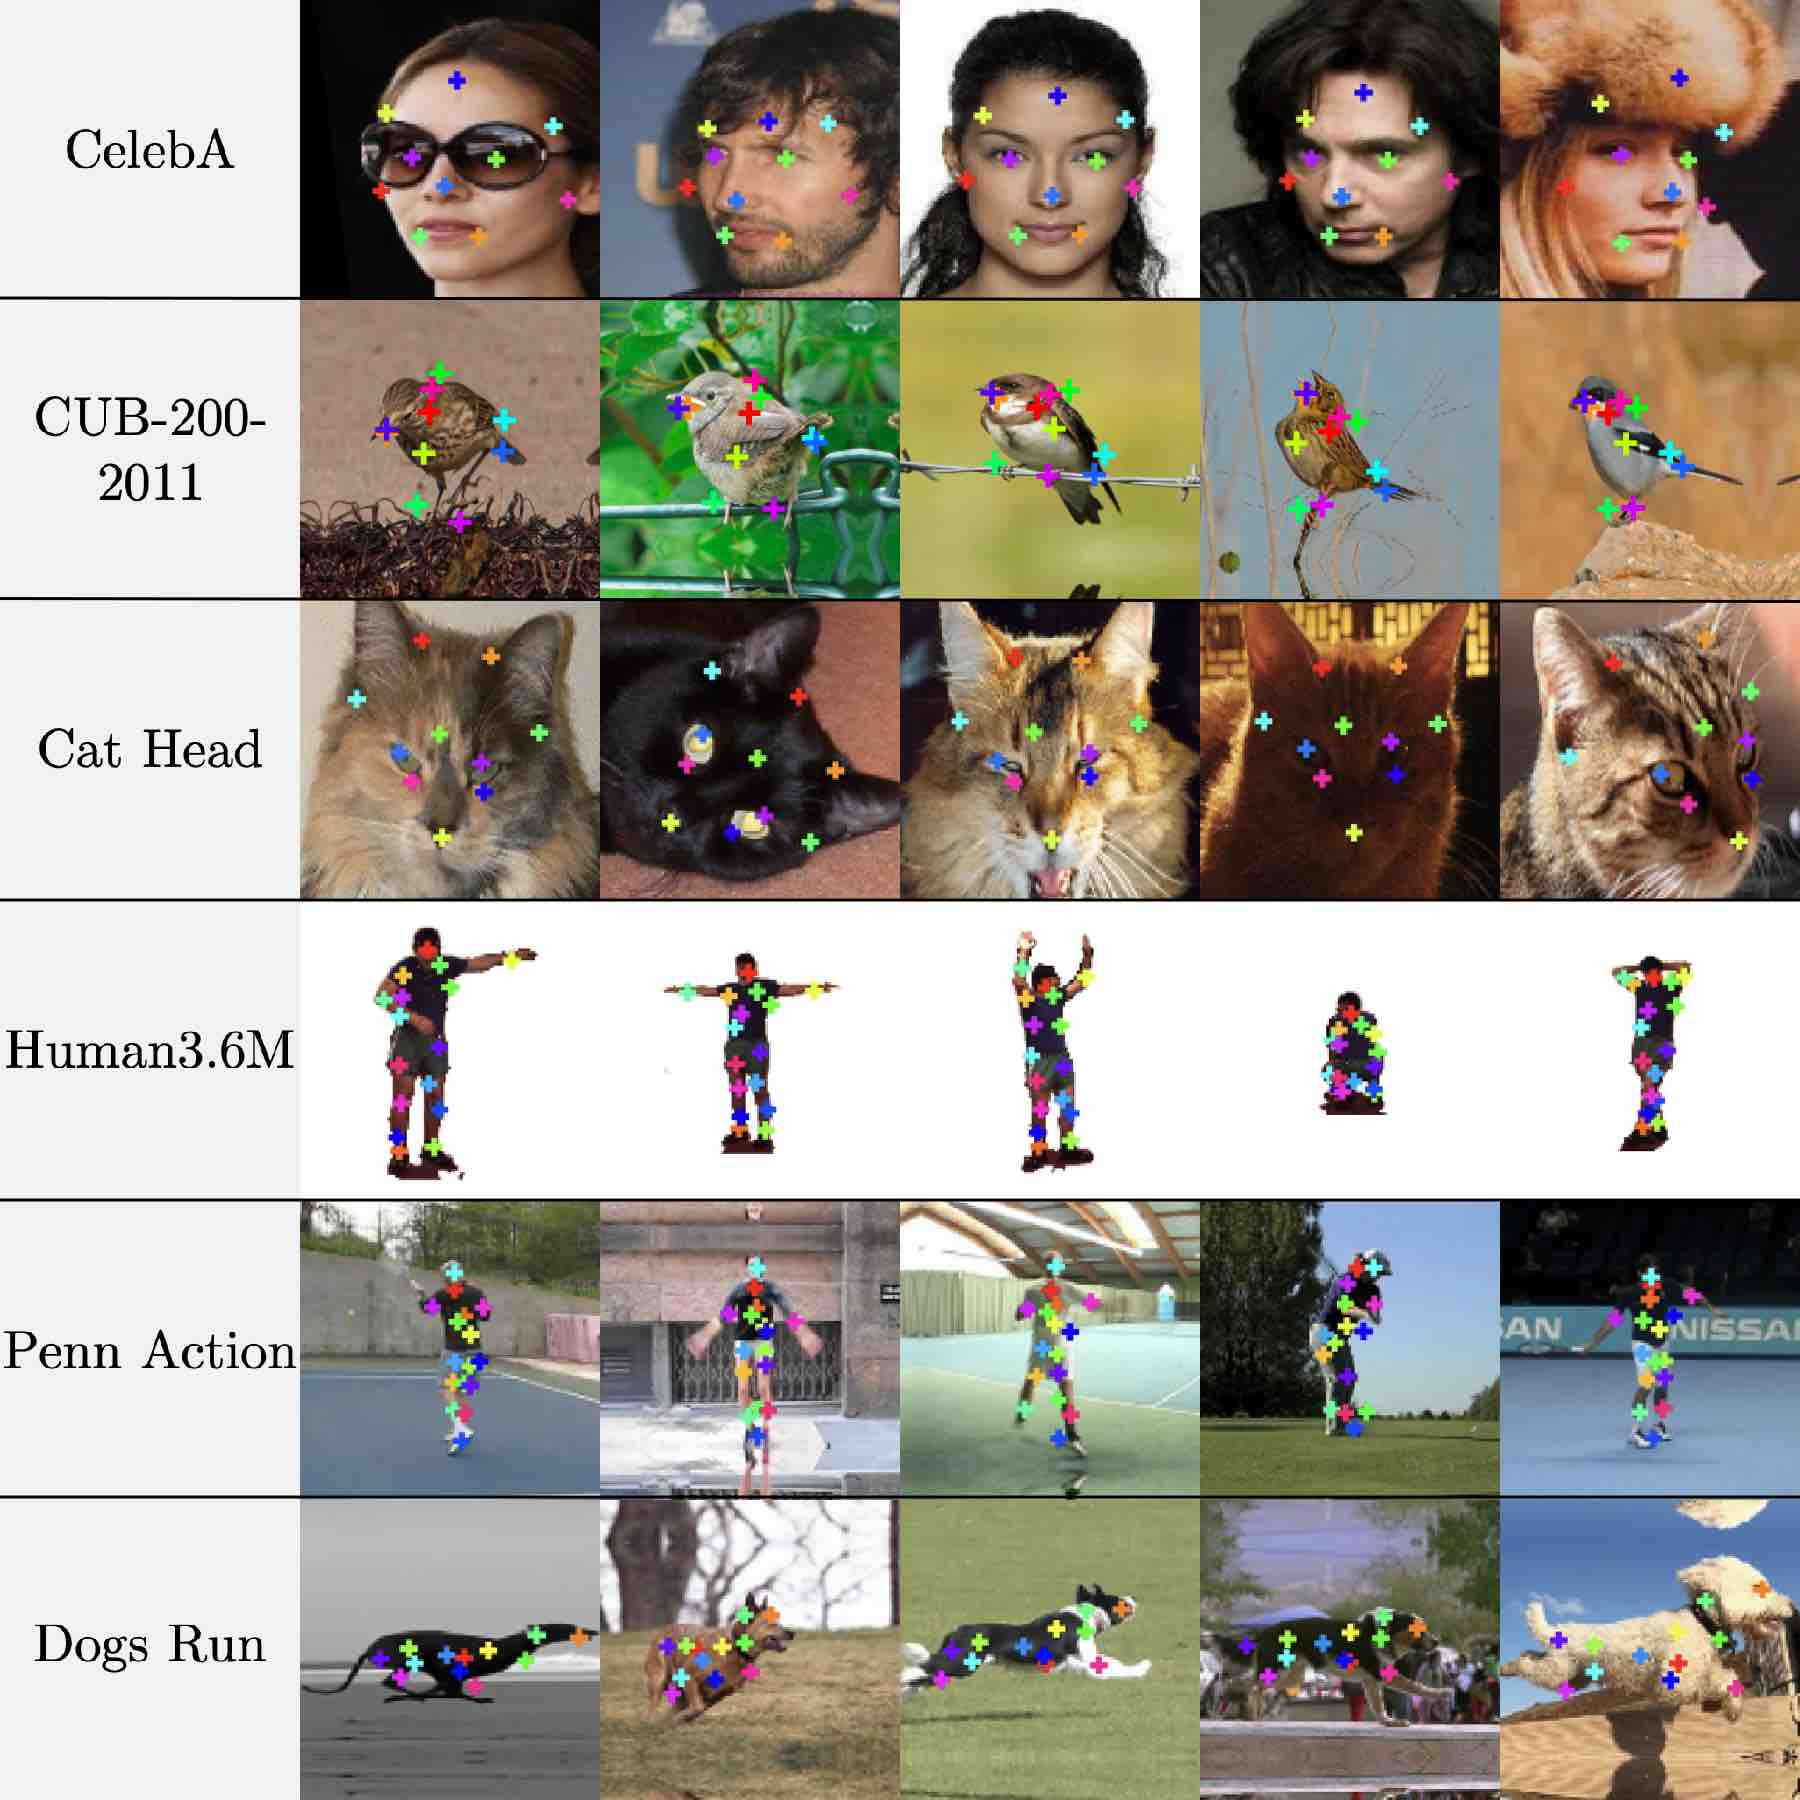
\includegraphics[trim={0cm 0cm 0cm 0cm},clip, width=1.\linewidth]{fig/kp_mania}
	\caption{{Unsupervised discovery of landmarks on diverse object classes such as human or cat faces and birds and for highly articulated human bodies and running dogs.}}
%	%(from CelebA, CUB-200-2011 and Cat Head)
%	and on articulated objects such as human bodies and running dogs.}}
	%(from Human3.6M (no background),  Penn Action (real world conditions) and Dogs Run).}}
	\label{fig:kp_mania}
\end{figure}
%
% AND COMPARISON TO ZHANG
% \begin{figure}[t]
	% \centering
	% \includegraphics[trim={0cm 0cm 0cm 0cm},clip, width=1.\linewidth]{mat/birds1x3}
	% \caption{{Comparison of regression results of our method (top row) to Zhang et al. \cite{Zhang:2018vz} (bottom row) on CUB-200-2011. The red dots mark the ground truth, the colored circles the regressed locations. The color coding is in terms of the error w.r.t the image edge length. (same visualization as in \cite{Zhang:2018vz})}}
	% \label{fig:compare}
% \end{figure}
\begin{figure}[t]
	\centering
	\includegraphics[trim={0cm 0cm 0cm 0cm},clip, width=1.\linewidth]{fig/birds1x3}
	\caption{Comparing discovered keypoints against \cite{Zhang:2018vz} on CUB-200-2011. We improve on object coverage and landmark consistency. Note our flexible part placement compared to a rather rigid placement of \cite{Zhang:2018vz} due to their part separation bias.}
	\label{fig:compare}
\end{figure}
% STATIC DATASETS: CELEBA, CATS, BIRDS
% \begin{table}[t]
	% \caption{{Comparison with other unsupervised methods for annotated landmark prediction on the Cat Head, MAFL (subset of CelebA), and CUB-200-2011 testing sets. The
	% error is given in \% of the inter-ocular distance for Cat Head and MAFL and in \% of the edge length of the image for CUB-200-2011.}}
	% \label{tab:static}
	% \centering
	% \begin{tabular}{l|ccccc}
	% \hline
	% Dataset & Cat Head &  & MAFL & & CUB\\
	  % \# Landmarks &10 & 20  & 10 & 30 &10  \\
	  % \hline
	 % Thewlis \cite{Thewlis:2017wi}
	 % & 26.76 & 26.94 & 6.32 & 5.76 & -  \\
	 % Jakab \cite{Jakab:2018wc}
	 % & - & - & 4.69 & \textbf{3.08} & - \\
	 % Zhang \cite{Zhang:2018vz}
	 % & 15.35 & 14.84 & 3.46 & 3.15 & 5.36 \\
	  % Ours & \textbf{9.88}  & \textbf{9.30} & \textbf{3.24} & 3.11 & \textbf{3.91}  \\ \hline  % image length is 600: 32.15 , 23.51
	% \end{tabular}
% \end{table}
\begin{table}[t]
	\caption{{Error of unsupervised methods for landmark prediction on the Cat Head, MAFL (subset of CelebA), and CUB-200-2011 testing sets.
	%For Cat Head and MAFL we report error in \% of inter-ocular distance, for CUB-200-2011 it is \% of edge length.
	The	error is in \% of inter-ocular distance for Cat Head and MAFL and in \% of edge length of the image for CUB-200-2011.}}
	\label{tab:static}
	\centering
	\begin{tabular}{l|cccc}
	\hline
	Dataset & Cat Head &  & MAFL & CUB\\
	  \# Landmarks &10 & 20  & 10 &10  \\
	  \hline
	 Thewlis \cite{Thewlis:2017wi}
	 & 26.76 & 26.94 & 6.32  & -  \\
	 Jakab \cite{Jakab:2018wc}
	 & - & - & 4.69 & - \\
	 Zhang \cite{Zhang:2018vz}
	 & 15.35 & 14.84 & 3.46 & 5.36 \\
	  Ours & \textbf{9.88}  & \textbf{9.30} & \textbf{3.24} & \textbf{3.91}  \\ \hline  % image length is 600: 32.15 , 23.51
	\end{tabular}
\end{table}
